\documentclass[11pt]{article}

\usepackage{epsfig}
\usepackage{amsfonts}
\usepackage{amssymb}
\usepackage{amstext}
\usepackage{amsmath}
\usepackage{xspace}
\usepackage{theorem}
\usepackage{times}
\usepackage{graphicx}

%\usepackage{layout}% if you want to see the layout parameters
                     % and now use \layout command in the body

% This is the stuff for normal spacing
\makeatletter
 \setlength{\textwidth}{6.5in}
 \setlength{\oddsidemargin}{0in}
 \setlength{\evensidemargin}{0in}
 \setlength{\topmargin}{0.25in}
 \setlength{\textheight}{8.25in}
 \setlength{\headheight}{0pt}
 \setlength{\headsep}{0pt}
 \setlength{\marginparwidth}{59pt}

 \setlength{\parindent}{0pt}
 \setlength{\parskip}{5pt plus 1pt}
 \setlength{\theorempreskipamount}{5pt plus 1pt}
 \setlength{\theorempostskipamount}{0pt}
 \setlength{\abovedisplayskip}{8pt plus 3pt minus 6pt}

 \renewcommand{\section}{\@startsection{section}{1}{0mm}%
                                   {2ex plus -1ex minus -.2ex}%
                                   {1.3ex plus .2ex}%
                                   {\normalfont\Large\bfseries}}%
 \renewcommand{\subsection}{\@startsection{subsection}{2}{0mm}%
                                     {1ex plus -1ex minus -.2ex}%
                                     {1ex plus .2ex}%
                                     {\normalfont\large\bfseries}}%
 \renewcommand{\subsubsection}{\@startsection{subsubsection}{3}{0mm}%
                                     {1ex plus -1ex minus -.2ex}%
                                     {1ex plus .2ex}%
                                     {\normalfont\normalsize\bfseries}}
 \renewcommand{\paragraph}{\@startsection{paragraph}{4}{0mm}%
                                    {1ex \@plus1ex \@minus.2ex}%
                                    {-1em}%
                                    {\normalfont\normalsize\bfseries}}
 \renewcommand{\subparagraph}{\@startsection{subparagraph}{5}{\parindent}%
                                       {2.0ex \@plus1ex \@minus .2ex}%
                                       {-1em}%
                                      {\normalfont\normalsize\bfseries}}
\makeatother

\newenvironment{proof}{{\bf Proof:  }}{\hfill\rule{2mm}{2mm}}
\newenvironment{proofof}[1]{{\bf Proof of #1:  }}{\hfill\rule{2mm}{2mm}}
\newenvironment{proofofnobox}[1]{{\bf#1:  }}{}
\newenvironment{example}{{\bf Example:  }}{\hfill\rule{2mm}{2mm}}
\renewcommand{\thesection}{\lecnum.\arabic{section}}

\renewcommand{\theequation}{\thesection.\arabic{equation}}
\renewcommand{\thefigure}{\thesection.\arabic{figure}}

\newtheorem{fact}{Fact}[section]
\newtheorem{lemma}[fact]{Lemma}
\newtheorem{theorem}[fact]{Theorem}
\newtheorem{definition}[fact]{Definition}
\newtheorem{corollary}[fact]{Corollary}
\newtheorem{proposition}[fact]{Proposition}
\newtheorem{claim}[fact]{Claim}
\newtheorem{exercise}[fact]{Exercise}

% math notations
\newcommand{\R}{\ensuremath{\mathbb R}}
\newcommand{\Z}{\ensuremath{\mathbb Z}}
\newcommand{\N}{\ensuremath{\mathbb N}}
\newcommand{\F}{\ensuremath{\mathcal F}}
\newcommand{\SymGrp}{\ensuremath{\mathfrak S}}

\newcommand{\size}[1]{\ensuremath{\left|#1\right|}}
\newcommand{\ceil}[1]{\ensuremath{\left\lceil#1\right\rceil}}
\newcommand{\floor}[1]{\ensuremath{\left\lfloor#1\right\rfloor}}
\newcommand{\poly}{\operatorname{poly}}
\newcommand{\polylog}{\operatorname{polylog}}

% asymptotic notations
\newcommand{\Oh}[1]{{\mathcal O}\left({#1}\right)}
\newcommand{\LOh}[1]{{\mathcal O}\left({#1}\right.}
\newcommand{\ROh}[1]{{\mathcal O}\left.{#1}\right)}
\newcommand{\oh}[1]{{o}\left({#1}\right)}
\newcommand{\Om}[1]{{\Omega}\left({#1}\right)}
\newcommand{\om}[1]{{\omega}\left({#1}\right)}
\newcommand{\Th}[1]{{\Theta}\left({#1}\right)}


% pseudocode notations
\newcommand{\xif}{{\bf{\em{if~}}}}
\newcommand{\xthen}{{\bf{\em{then~}}}}
\newcommand{\xelse}{{\bf{\em{else~}}}}
\newcommand{\xelseif}{{\bf{\em{elif~}}}}
\newcommand{\xfi}{{\bf{\em{fi~}}}}
\newcommand{\xcase}{{\bf{\em{case~}}}}
\newcommand{\xendcase}{{\bf{\em{endcase~}}}}
\newcommand{\xfor}{{\bf{\em{for~}}}}
\newcommand{\xto}{{\bf{\em{to~}}}}
\newcommand{\xby}{{\bf{\em{by~}}}}
\newcommand{\xdownto}{{\bf{\em{downto~}}}}
\newcommand{\xdo}{{\bf{\em{do~}}}}
\newcommand{\xrof}{{\bf{\em{rof~}}}}
\newcommand{\xwhile}{{\bf{\em{while~}}}}
\newcommand{\xendwhile}{{\bf{\em{endwhile~}}}}
\newcommand{\xand}{{\bf{\em{and~}}}}
\newcommand{\xor}{{\bf{\em{or~}}}}
\newcommand{\xerror}{{\bf{\em{error~}}}}
\newcommand{\xreturn}{{\bf{\em{return~}}}}
\newcommand{\xparallel}{{\bf{\em{parallel~}}}}
\newcommand{\T}{\hspace{0.5cm}}
\newcommand{\m}{\mathcal}

\def\sland{~\land~}
\def\slor{~\lor~}
\def\sRightarrow{~\Rightarrow~}

\def\comment#1{\hfill{$\left\{\textrm{{\em{#1}}}\right\}$}}
\def\lcomment#1{\hfill{$\left\{\textrm{{\em{#1}}}\right.$}}
\def\rcomment#1{\hfill{$\left.\textrm{{\em{#1}}}\right\}$}}
\def\fcomment#1{\hfill{$\textrm{{\em{#1}}}$}}
\def\func#1{\textrm{\bf{\sc{#1}}}}
\def\funcbf#1{\textrm{\textbf{\textsc{#1}}}}

\newcommand{\hide}[1]{}

\newcommand{\prob}[1]{\ensuremath{\text{{\bf Pr}$\left[#1\right]$}}}
\newcommand{\expct}[1]{\ensuremath{\text{{\bf E}$\left[#1\right]$}}}
\newcommand{\Event}{{\mathcal E}}

\newcommand{\mnote}[1]{\normalmarginpar \marginpar{\tiny #1}}

\makeatletter
   \newcommand\figcaption{\def\@captype{figure}\caption}
   \newcommand\tabcaption{\def\@captype{table}\caption}
\makeatother


%%%%%%%%%%%%%%%%%%%%%%%%%%%%%%%%%%%%%%%%%%%%%%%%%%%%%%%%%%%%%%%%%%%%%%%%%%%
% Document begins here %%%%%%%%%%%%%%%%%%%%%%%%%%%%%%%%%%%%%%%%%%%%%%%%%%%%
%%%%%%%%%%%%%%%%%%%%%%%%%%%%%%%%%%%%%%%%%%%%%%%%%%%%%%%%%%%%%%%%%%%%%%%%%%%

\newcommand{\headings}[4]{
{\bf CSE548 \& AMS542: Analysis of Algorithms, Fall 2017} \hfill {{\bf Lecturer:} #1}\\
{{\bf Topic:} #2} \hfill {{\bf Date:} #3} \\
{{\bf Scribe:} #4}\\
\rule[0.1in]{\textwidth}{0.025in}
%\thispagestyle{empty}
}

\begin{document}

\headings{Dr. Rezaul A Chowdhury}{Master Theorem Contd. \& Akra-Bazzi Recurrences}{25 September 2017}{Raghunandana Jayarama Reddy}
\newcommand{\lecnum}{8}  % Lecture Number

\section{Master Theorem \lecnum}

    $$
	T(n) = \left\{
        \begin{array}{ll}
        		\Th{1}, & \quad n \leq 1, \\
            aT(\frac{n}{b}) + f(n), & otherwise(a \geq 1\ and\ b > 1).
        \end{array}
    \right.     
	$$
    
{\bf case 1 }: If f(n) = O(n$^{log_{b}a-\epsilon}$) for some constant $\epsilon >$ 0, then \textit{T(n) =     $\Theta(n^{log_{b}a})$} \\
{\bf case 2 }: If f(n) = $\Theta$(n$^{log_{b}a} lg^{k} n $), then \textit{T(n) = $\Theta(n^{log_{b}a} lg^{k+1} n)$} \\
{\bf case 3 }: If f(n) = $\Omega($n$^{log_{b}a+\epsilon}$) for some constant $\epsilon >$ 0, and if \textit{a f$\biggl(\dfrac{n}{b}\biggr)$} $\leq$ \textit{cf(n)} for some constant  \textit(c) $<$ 1 and all sufficiently large \textit(n), then \textit{T(n) = $\Theta$(f(n)))} \\

\begin{figure}[h!] 
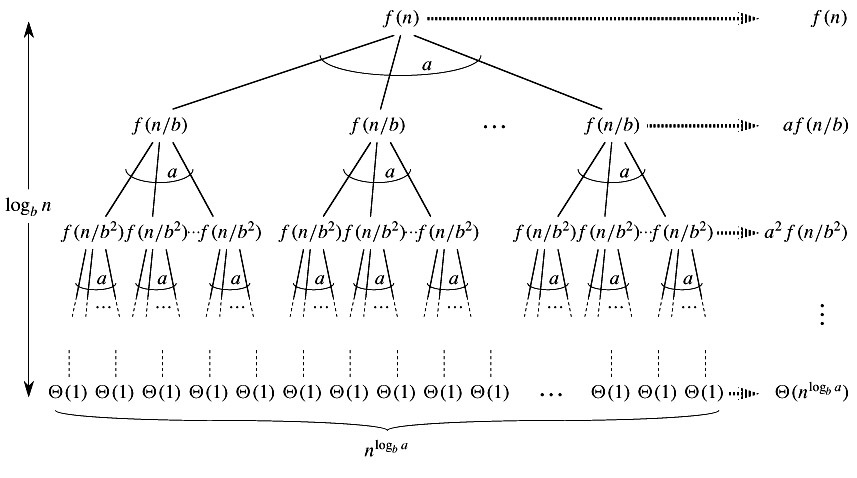
\includegraphics[width=0.9\linewidth]{RecurseTree.jpg}
\caption{\small \sl Recurrence Tree \label{fig:Recurrence Tree}}
\end{figure}


\subsection {Recurrences not solvable using the Master theorem}

{\bf Example 1:} T(n) = $\sqrt{n}$ T $\biggl(\dfrac{n}{2}\biggr)$ + n 
According to the Master's Theorem, here a = $\sqrt{n}$ is not a constant \\
{\bf Example 2:} T(n) = 2T$\biggl(\dfrac{n}{log_{}n}\biggr)$ + ${n^{2}}$
In this example, $b = log_{}n$ is not a constant\\
{\bf Example 3:} T(n) = ${{1} \over  {2}}$T$\biggl(\dfrac{n}{2}\biggr)$ + ${n^{2}}$
In this example, a(number of subproblems should be atleast 1) = ${{1} \over  {2}}$ is not $ \geq 1 $ \\
{\bf Example 4:} T(n) = 2T$\biggl(\dfrac{4n}{3}\biggr)$ + n
Here, b(subproblem size) = ${{3} \over  {4}}$ is not $ > 1$ \\
{\bf Example 5:} T(n) = 3T$\biggl(\dfrac{n}{2}\biggr)$ - n
Here, f(n) = -n is not positive. \\ 
{\bf Example 6:} T(n) = 2T$\biggl(\dfrac{n}{2}\biggr)$ + $n^2 \sin n$
Here, f(n) = $n^2 \sin n$ and $\sin n $ range varies from -1 to 1 for any given n. Hence violates the regularity condition of case 3. \\
{\bf Example 7:} T(n) = 2T$\biggl(\dfrac{n}{2}\biggr)$ + $\biggl(\dfrac{n}{log_{}n}\biggr)$
In the above example, \\
No. of leaves, n$^{log_{b}a}$ = n$^{log_{2}2}$ = n.\\
With case 1, f(n) = O(n$^{log_{b}a}$) = $\biggl(\dfrac{n}{log_{}n}\biggr)$, but $ \neq $ O(n$^{log_{b}a-\epsilon}$) for any constant $\epsilon >$ 0. \\
With case 2, f(n) = $\Theta$(n$^{log_{b}a} lg^{k} n $)  Here, f(n) = $n{log^-{1}_{}n}$ where k = -1 is not $\geq 0$ to solve. \\
With case 3, f(n) = $\Omega($n$^{log_{b}a+\epsilon}$) for any constant $\epsilon >$ 0, which infers that if f(n) is polynomially lesser than the number of leaves we can solve it but the given f(n) value doesn't indicate any specific range as it is a logarithmic function over some value n.\\
Hence, this cannot be solved by master's theorem.\\
{\bf Example 8:} T(n) = T$\biggl(\dfrac{n}{2}\biggr)$ + 2T$\biggl(\dfrac{n}{4}\biggr)$ + n.
Master's theorem can be applied for only one set of 'a' and 'b' values (Means a definitive set of branching)
Here, a and b values are not fixed and hence cannot be solved by Master's theorem.\\



{\bf Thus we realized that many divide and conquer problems cannot be solved by Master's theorem. Thus we will learn an extension which is a generalization of Master's theorem called the Akra-Bazzi recurrence solution.}\\

Before learning Akra-Bazzi recurrences, to provide an intuition of the Master's theorem, lets see if Master's theorem can be written in a different form.

Let's consider Master Theorem,\\
\begin{align*}
T(n) =& \Theta(n^{\log_a b}) + \sum_{j=0}^{\log_b n - 1} {a^{j}}f\left(\frac{n}{b^{j}}\right) 
\end{align*}

Here,\\ 

n$^{log_{b}a}$ = Number of Leaves in all the levels.\\
g(n) = $\sum_{j=0}^{\log_b n - 1} {a^{j}}f\left(\frac{n}{b^{j}}\right)$ = cost of division and merging of all the levels combined. i.e., from 0 to (n-1) levels.\\
$a^{j}$ is the number of subproblems at that level\\
$f\left(\frac{n}{b^{j}}\right)$ is the function that denotes the cost of dividing and merging of subproblems at each level.

\begin{proof}
$T(n)$ = $(n^{\log_a b}) + \sum_{j=0}^{\log_b n - 1} {a^{j}}f\left(\frac{n}{b^{j}}\right)$

Let us assume that p = ${\log_a b}$ \\
Input size at level j, ${n_j}$ = $\frac{n}{b^{j}}$

Now, $T(n)$ = $(n^p) + \sum_{j=0}^{\log_b n - 1} {a^{j}}f\left(n_j\right)$

Let us consider $\sum_{j=0}^{\log_b n - 1} {a^{j}}f\left(n_j\right)$ which we can write in different form to generalize, \\

\centering Since p = ${\log_a b}$ ,\\
 a = ${b^{p}}$\\
 $a^{j}$ = ${({b^{p}})^j}$ = ${({b^{j}})^p}$ \\
 $a^{j}$ = ${\biggl(\frac{n}{\frac{n}{b^{j}}}\biggr)^{p}}$ \\ 
 $a^{j}$ = ${\biggl(\frac{n}{n^{j}}\biggr)^{p}}$ \\
 
 This represents the number of subproblems at level j.
 
 Now, $\sum_{j=0}^{\log_b n - 1} {a^{j}}f\left(n_j\right)$ = $\sum_{j=0}^{\log_b n - 1} {{\biggl(\frac{n}{n^{j}}\biggr)^{p}}}f\left(n_j\right)$ 
 
 Here, $n_j$ takes log n different values based on j\\
 For every recursion level(lets say 'm') which varies from nth level to the last level, lets say 1( since merging and computation starts from that level) \\
 
 Now, $\sum_{j=0}^{\log_b n - 1} {{\biggl(\frac{n}{n^{j}}\biggr)^{p}}}f\left(n_j\right)$ = $\sum_{m \epsilon \{ b , b^{2} , . . . ,\frac{n}{b^{2}},\frac{n}{b}, n \}} {{\biggl(\frac{n}{m}\biggr)^{p}}}f\left(m \right)$ 
 
 Since, $n^{p}$ is not changing with respect to the summation,\\
 $\sum_{m \epsilon \{ b , b^{2} , . . . ,\frac{n}{b^{2}},\frac{n}{b}, n \}} {{\biggl(\frac{n}{m}\biggr)^{p}}}f\left(m \right)$ =  $n^{p} \sum_{m \epsilon \{ b , b^{2} , . . . ,\frac{n}{b^{2}},\frac{n}{b}, n \}} \frac{f\left(m \right)}{m^{p}}$ \\
 
For some recursion level m, lets consider the function f(m), \\
In each level, $\{ b , b^{2} , . . . ,\frac{n}{b^{2}},\frac{n}{b}, n \}$  n changes by a constant factor b, and hence f(m) also changes by a constant factor.\\
where, f(m) =$ \theta ( f(n)) $  \\

For one level, $\sum_{m=n} {\frac{f\left(m \right)}{m^{p}}}  \rightarrow  \sum_{m={\frac{n}{b}}+1} {\frac{f\left(m \right)}{m^{p}}}$ 

From the above inference, 
$\sum_{m={\frac{n}{b}}+1}^{n} {\frac{f\left(m \right)}{m^{p}}}$ = $ \theta \biggl(\sum_{m={\frac{n}{b}}+1} {\frac{f\left(n \right)}{n^{p}}}\biggr) $\\

Here, the factor ${\frac{f\left(n \right)}{n^{p}}} $ is a constant and not dependent of change factor m.

Therefore, $ \theta \biggl(\sum_{m={\frac{n}{b}}+1} {\frac{f\left(n \right)}{n^{p}}}\biggr) $ = $ \theta \biggl((n - \frac{n}{b} -1 + 1 {\frac{f\left(n \right)}{n^{p}}}\biggr) $ \\ 

= $ \theta \biggl(n(1 - \frac{1}{b})  {\frac{f\left(n \right)}{n^{p}}}\biggr) $ \\ 

For large values of b, $(1 - \frac{1}{b})$ will be 1\\
This implies, $\sum_{m={\frac{n}{b}}+1}^{n} {\frac{f\left(m \right)}{m^{p}}}$ = $ \theta \biggl(n  {\frac{f\left(n \right)}{n^{p}}}\biggr) $ \\
 From the above inference $\sum_{m=n} {\frac{f\left(m \right)}{m^{p}}}  \rightarrow  \sum_{m={\frac{n}{b}}+1} {\frac{f\left(m \right)}{m^{p}}}$,\\ 
 $\sum_{m={\frac{n}{b}}+1}^{n} {\frac{f\left(m \right)}{m^{p}}}$ = $ \theta \biggl(n  \sum_{m=n} {\frac{f\left(m \right)}{m^{p}}}\biggr) $ \\
  which can be written as,\\
  $\sum_{m=n} {\frac{f\left(m \right)}{m^{p}}}$ = $ \theta \biggl(\frac{1}{n}  \sum_{m={\frac{n}{b}}+1} {\frac{f\left(m \right)}{m^{p}}}\biggr) $ \\
  
 = $ \theta \biggl(\sum_{m={\frac{n}{b}}+1} {\frac{f\left(m \right)}{m^{(p+1)}}}\biggr) $ \\
 
 Thus,$\sum_{j=0}^{\log_b n - 1} {{\biggl(\frac{n}{n^{j}}\biggr)^{p}}}f\left(n_j\right)$ = $ \theta \biggl( (n^p)  \sum_{m=1}^{n} {\frac{f\left(m \right)}{m^{(p+1)}}}\biggr) $ \\

\end{proof}

 Thus we came to a conclusion that in a complicated recurrence equation which has multiple a and b values can be solved in the above way which is very similar to akra-bazzi reference solution.
 



\section{Akra-Bazzi Recurrences} 
 
By Master's theorem,
T(n) = $\theta {(n^{p})}$ for some value p which is $ log_{b}{a} $

Let us consider a complex recurrence equation which has multiple a and b and does not have f(n),\\
T(n) = $a_1 T \biggl(\frac{n}{b_1}\biggr) + a_2 T \biggl(\frac{n}{b_2}\biggr) + a_3 T \biggl(\frac{n}{b_3}\biggr) $ \\ 

T(n) = $a_1 \biggl(\frac{n}{b_1}\biggr)^{p} + a_2  \biggl(\frac{n}{b_2}\biggr)^{p} + a_3  \biggl(\frac{n}{b_3}\biggr)^{p} $ \\

T(n) = $\biggl(\frac{a_1}{b_1} + \frac{a_2}{b_2} + \frac{a_3}{b_3} \biggr) * (n)^{p} $

By Master's theorem, $\biggl(\frac{a_1}{b_1} + \frac{a_2}{b_2} + \frac{a_3}{b_3} \biggr) =1 $ \\

This complex equation can be solved by finding a value of p for which $\biggl(\frac{a_1}{b_1} + \frac{a_2}{b_2} + \frac{a_3}{b_3} \biggr) =1 $ \\

But if there is a cost of dividing and merging, i.e., f(n) in the equation then the above solution doesn't work. 



\subsection{Deterministic select}

{Input:}  An array A[q:r] of distinct elements, and integer $k \epsilon [1,r-q + 1]$  \\
{Output:} An element x of A[q:r] such that rank(x,A[q:r]) = k 

We want to find the kth smallest number here.

Algorithm:

\begin{itemize}
\item Let $n \leq 140 $ some constant, for reference lets consider some value 140. Then sort the numbers of the array less than that  constant. Here, it takes time complexity of $\theta (1) $.
\item Otherwise if n is very large. Divide the array into groups of 5. Each group is of size similar to $\frac{n}{5}$.
\item Then find the median of all those 5 groups.
\item Now find the median of those 5 medians. Use the algorithm recursively to find the median of 5 medians.
\item Do the recursive solving with the bi-partition median method.
\end{itemize}
This select method reduces the time complexity to solve the problem to a factor of $n$. 




\begin{figure}[h!]  
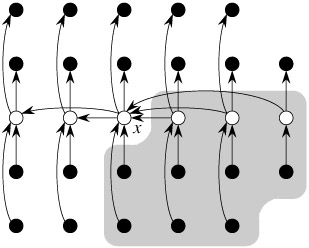
\includegraphics[width=0.9\linewidth]{Median.jpg}
\caption{\small \sl SELECT(A,k) \label{fig:DeterministicSelect}}
\end{figure}
$SELECT(A,k)$ : Given an unsorted set A of $n(=|A|)$ items, find the $k^{th}$ smallest item in the set.

\begin{itemize}
\item All the items are arranged according to the values of the medians in the groups.
\item $x$ is the median of medians of the groups.
\item At least half of the group is to the left of $x$ and other to the right.
\item Amongst the left half atleast half(indicated in green) are smaller than $x$ and the other half of right half (indicated in blue) are larger than $x$. Cant say anything for the other elements outside the blue and green groups.
\item Intuitively the items definitely smaller than $x$ is $ \geq 3 \biggl((\frac{1}{2}) (\frac{n}{5}) - 1 \biggr)$ $ \geq \biggl(\frac{3n}{10} - 6 \biggr)$
\item the items definitely larger than $x$ is $ \geq 3 \biggl((\frac{1}{2}) (\frac{n}{5}) - 1 \biggr)$ $ \geq \biggl(\frac{3n}{10} - 6 \biggr)$
\item Thus the items in any recursive call $ \leq n - \biggl(\frac{3n}{10} - 6\biggr) $
\item $  n - \biggl(\frac{3n}{10} - 6\biggr) $ = $ \biggl(\frac{7n}{10} + 6\biggr) $ which are the maximum number of elements on the other side. 
\item Thus the level of computations reduce by an order of 7.
\end{itemize}


Consider the following recurrence which describes the worst-case running time of the deterministic selection algorithm.

	 $$
	T(n) \leq  \left\{
        \begin{array}{ll}
        		\theta{1}, & \quad if \T n < 140 , \\
            T(\ceil{\frac{n}{5}}) + T \biggl(\frac{7n}{10} + 6 \biggr) + \theta(n) , &  \T if\T n \geq 140.
        \end{array}
    \right.     
	$$

Here, $T(\ceil{\frac{n}{5}})$ is the Time complexity of one median amongst a group of 5. 

For a large value of n,
$\frac{8n}{10} \geq \biggl(\frac{7n}{10} + 6 \biggr) $ 

By simplifying, $ n \geq 60 $.

This assumption is based on the only case where $n$ is sufficiently larger.

Thus we obtain the following upper bound for T(n), 

	 $$
	T'(n) =  \left\{
        \begin{array}{ll}
        		\theta{1}, & \quad if \T n < 140 , \\
            T'({\frac{n}{5}}) + T' \biggl(\frac{8n}{10} \biggr) + \theta(n) , &  \T if\T n \geq 140.
        \end{array}
    \right.     
	$$
    
If we consider, $\frac{7.5n}{10} \geq \biggl(\frac{7n}{10} + 6 \biggr) $ 

By simplifying, $ n \geq 120 $.
    
Thus we obtain the following upper bound for T(n), 

	 $$
	T''(n) =  \left\{
        \begin{array}{ll}
        		\theta{1}, & \quad if \T n < 140 , \\
            T''({\frac{n}{5}}) + T'" \biggl(\frac{7.5n}{10} \biggr) + \theta(n) , &  \T if\T n \geq 140.
        \end{array}
    \right.     
	$$    
    
Thus we need Akra-Bazzi recurrence solution for solving complex recurrences like the above.

\clearpage
\end{document}
